\noindent \textred{3.} 
\textbf{(3 points)} \textit{Improving the FashionMNIST classifier}. In the \href{https://github.com/kvgarimella/dl-demos/blob/main/demo01-basics.ipynb}{\underline{first demo}}, we trained a simple logistic regression model to classify MNIST digits. Repeat the same experiment, but now use a (dense) neural network with three (3) hidden layers with 256, 128, and 64 neurons respectively, all with ReLU activations. Display train- and test- loss curves, and report test accuracies of your final model. You may have to tweak the total number of training epochs to get reasonable accuracy. Finally, draw any 3 image samples from the test dataset, visualize the predicted class probabilities for each sample, and comment on what you can observe from these plots.
\\
\noindent \myAnswer{
The whole PDF exported from Jupyter notebook is attached at the end. The improved dense neural network was trained for 20 epochs with learning rate of $1\times 10^{-2}$. Below is the loss and accuracy curve. After training, both training and testing accuracy achieved $> 85\%$.
\begin{figure}[!h]
    \centering
    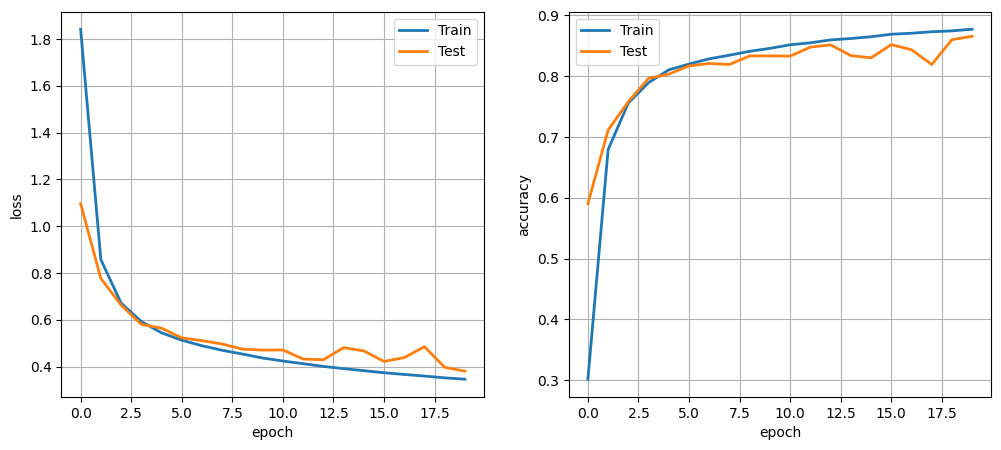
\includegraphics[width=0.8\linewidth]{HWs/HW1/figures/3-1.png}
    \vspace{-10pt}
\end{figure}
\\
Below is the plot of 3 randomly selected samples from the test set with their true labels and predicted results. We can see that most results are correct. Even though the third sample was incorrectly predicted, its prediction still had some components on the true label, \ie, category 0. What's more, the wrongly predict class 6 is ``Shirt", which is close to the true label 0 ``T-Shirt". Therefore, the results are reasonable and interpretable.
\begin{figure}[!h]
    \centering
    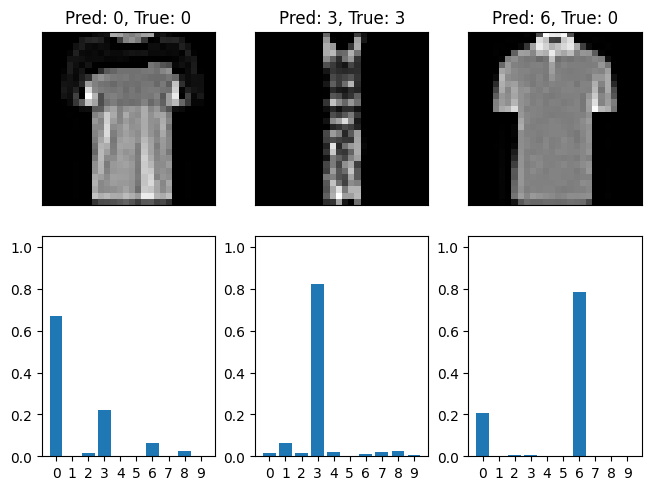
\includegraphics[width=0.7\linewidth]{HWs/HW1/figures/3-2.png}
\end{figure}
}